\chapter{TUTORIAL}
\label{tutorial}
Aqui será ensinado como utilizar este modelo, e de forma geral a utilizar o LaTeX. Leia brevemente este tutorial para aprender o básico de como utilizar o LaTeX.
\section{CONHECENDO}
\label{conhecendo}
O LaTeX é um sistema de preparação de documentos. O escritor usa o texto simples, ao invés do formatado, como em processadores de texto \textit{What You See Is What You Get}, WYSIWYG, onde o usuário vê o texto já formatado.

\section{INSTALAÇÃO}
\label{instalacao}
Para usuários do Windows, o LaTeX encontra-se disponível de forma ampla através de diversos editores e distribuidores. Este tutorial indica a utilização da distribuição MiKTeX, disponível em \url{https://miktex.org/download} e do editor TexMaker, disponível em \url{https://www.xm1math.net/texmaker/download.html}. A instalação é simples.

\section{INICIANDO}
\label{iniciando}
Para começar a escrever em LaTeX, é necessário executar o arquivo
\verb|uniguatex-tcc| disponível na pasta da Uniguatex. Neste arquivo encontra-se a ordem do documento que será criado. Se quiser omitir algo, basta incluir o símbolo de porcentagem, antes do item. Este processo é chamado de comentar uma linha, ou seja, tudo o que for colocado com este símbolo antes será um comentário e não uma ação que deverá ser executada.//

\begin{verbatim}
%%**********************************************%
%			LISTA DE QUADROS				   %                      
%**********************************************%
\renewcommand{\listofquadroname}{LISTA DE QUADROS}
\renewcommand{\cftdotsep}{1}
\pdfbookmark[0]{\listofquadroname}{loq}
\listofquadro*
\cleardoublepage
\end{verbatim}//

Para iniciar este documento, comente a linha de orientações, desta forma,//
\begin{verbatim}
%include{2-textual/orientacoes}
\end{verbatim}//
Pronto, agora é só entrar em cada arquivo do LaTeX e digitar seu Trabalho de Conclusão de Curso.

\section{ENTENDENDO}
\label{entendendo}
Em um documento LaTeX estão contidos diversas linhas de códigos e de ações que irão criar o texto final.
Para iniciar um arquivo, é criado um comando de tipo de documento. Ele é facilmente encontrado no início do uniguatex-tcc,
\begin{verbatim}
\documentclass[oneside]{uniguatex}
\end{verbatim}

\section{ESCREVENDO}
\label{escrevendo}

\subsection{Parâmetros Iniciais}
\label{parametrosiniciais}
Para iniciar a escrita é necessário ir até a primeira pasta, indicada por 1-pretextual. Nesta pasta existem arquivos Pré-Textuais do TCC, de capa e folha de rosto, às listas e ao sumário. As listas, com exceção da lista de siglas, que está sendo trabalhada no momento, são geradas automaticamente, não sendo necessário alterar nada.
A capa é o primeiro item de alteração, que contém nome do autor, título do projeto, curso e orientador. Ao abrir este arquivo, uma página irá aparecer mostrando itens que devem ser mudados. Para alterar este item, insira o texto desejado entre chaves \verb|{ }|. Desta forma,

\begin{verbatim}
\titulo{Titulo do Trabalho} % alterar o título do trabalho
\autor{Nome Completo do Autor} % alterar o nome do autor
\end{verbatim}

Deverão ser alterados para satisfazer o trabalho acadêmico.
Além disto, são utilizados diversos pacotes para que seja possível visualizar o documento final, bem como de editar partes específicas do texto, como inclusão de mídias gráficas e de cores.

\subsection{Escrita}
\label{escrita}

Todo documento LaTeX é iniciado em sua escrita através do comando \verb|\begin{document}|, onde tudo o que o autor escrever estará abaixo desta linha. Para finalizar é necessário encerrar este comando, com \verb|\end{document}|.
Em geral, todos os comandos são dados desta forma, com o início e o fim. Desta forma, para todos os comandos necessários, dá-se esta codificação, em \verb|begin{}| e \verb|end{}|.

\subsubsection{Formas de Escrita}
\label{formasdeescrita}
Para se utilizar de texto em negrito, utiliza-se:
\verb|\textbf{ Texto em negrito }|, desta forma, se produzirmos uma frase que contenha alguma palavra em negrito, teremos:

\begin{verbatim}
\Devemos utilizar o LaTeX da \textbf{melhor} forma
\end{verbatim}

Gerando a frase:
Devemos utilizar o LaTeX da \textbf{melhor} forma.

O mesmo acontece com texto em itálico, sublinhado, entre outros.

\begin{verbatim}
A \textit{grama} do \underline{vizinho} é \textbf{verde}.
\end{verbatim}

A \textit{grama} do \underline{vizinho} é \textbf{verde}.

Caracteres em branco são caracterizados como espaços pelo LaTeX.
Uma linha em branco entre dois textos, ou linhas de texto delimita o fim de um parágrafo.
Vários caracteres em branco, ou várias linhas em branco, delimitam apenas um único espaço em branco ou linha de final de parágrafo.

Alguns símbolos são caracteres especiais de codificação do LaTeX, desta forma, para solicitar este na escrita, utiliza-se da seguinte maneira.
\begin{multicols}{2}
\footnotesize
\begin{verbatim}
\# \$ \% \^{} \& \_ 
\{ \} \~{} \textbackslash
\end{verbatim}
\# ~ \$ ~ \% ~ \^{} ~ \& ~ \_ \\
\{ ~ \} ~ \~{} ~ \textbackslash
\end{multicols}

\subsubsection{Alinhamento}
\label{alinhamento}
Alinhamento funciona de acordo com o que já foi visto, com o comando de início e fim.
Desta forma, para alinharmos o texto à esquerda, direita ou centralizado, usamos:
\begin{verbatim}
\begin{flushleft}
Texto alinhado à esquerda
\end{flushleft}

\begin{flushright}
Texto alinhado à direita
\end{flushright}

\begin{center}
Texto centralizado
\end{center}
\end{verbatim}

\begin{flushleft}
Texto à esquerda
\end{flushleft}

\begin{flushright}
Texto à direita
\end{flushright}

\begin{center}
Texto centralizado
\end{center}

\subsection{Listas}
\label{listas}
Listas enumerads dentro do texto podem ser obtidas através de comandos de início e fim.
\begin{verbatim}
\begin{enumerate}
\item 5 Beterrabas
\item 2 Cenouras
\item 5 Ovos
\end{enumerate}
\end{verbatim}

O resultado é:

\begin{enumerate}
\item 5 Beterrabas
\item 2 Cenouras
\item 5 Ovos
\end{enumerate}

Listas de itens utilizam o comando:

\begin{verbatim}
\begin{itemize}
\item 5 Beterrabas
\item 2 Cenouras
\item 5 Ovos
\end{itemize}
\end{verbatim}

E o resultado é:

\begin{itemize}
\item 5 Beterrabas
\item 2 Cenouras
\item 5 Ovos
\end{itemize}

Além disto, listas aninhadas podem ser criadas.

\begin{verbatim}
\begin{itemize}
    \item Alumínio
    \item Aço
    \begin{itemize}
        \item Aço 1020
        \item Aço 1045
        \item Aço 1080
    \end{itemize}
    \item Cobre
\end{itemize}
\end{verbatim}

Como resultado, tem-se:

\begin{itemize}
    \item Alumínio
    \item Aço
    \begin{itemize}
        \item Aço 1020
        \item Aço 1045
        \item Aço 1080
    \end{itemize}
    \item Cobre
\end{itemize}

E lista aninhadas enumeradas, são escritas da seguinte forma:

\begin{verbatim}
\begin{enumerate}
    \item Terremotos
    \begin{enumerate}
        \item Naturais
        \item Induzidos
    \end{enumerate}
    \item Furacões
    \begin{enumerate}
        \item Categoria 1
        \item Categoria 2
        \item Categoria 3
    \end{enumerate}
    \item Vulcões 3
    \begin{enumerate}
        \item de Escudo
        \item Cúpulas de Lava
        \item Cones de Cinza
        \item Submarinos
    \end{enumerate}
\end{enumerate}
\end{verbatim}

E como resultado, a lista criada será:

\begin{enumerate}
    \item Terremotos
    \begin{enumerate}
        \item Naturais
        \item Induzidos
    \end{enumerate}
    \item Furacões
    \begin{enumerate}
        \item Categoria 1
        \item Categoria 2
        \item Categoria 3
    \end{enumerate}
    \item Vulcões 3
    \begin{enumerate}
        \item de Escudo
        \item Cúpulas de Lava
        \item Cones de Cinza
        \item Submarinos
    \end{enumerate}
\end{enumerate}

\subsection{Tabelas}
O comando tabular é utilizado para criar tabelas dentro do LaTeX, onde \verb|\begin{tabular}| inicia o processo e \verb|\end{tabular}| encerra o mesmo.

\begin{verbatim}
\begin{tabular}{|c|c|}
\hline
Abacaxi & R\$2,63\\
\hline
Laranja & R\$1,29\\
\hline
\end{tabular}
\end{verbatim}

Note que após o início do comando tabular existe \textbf{{|c|c|}}. Este comando delimita que deverão ser criadas linhas para as colunas, em \textbf{|} e o que for inserido deve ser centralizado, \textbf{c}. Desta forma, a tabela criada terá três linhas divisórias verticais e duas colunas.
Dentro deste ambiente, alguns símbolos dão comandos para avançar coluna, criar linha e inserir dados.
O símbolo \verb|&| avança uma coluna, ou seja, insere dados na próxima cédula.
O símbolo \verb|//| inicia uma nova linha.
O código \verb|\hline| insere uma linha divisória horizontal.
A tabela gerada é expressa abaixo.

\begin{tabular}{|c|c|}
\hline
Abacaxi & R\$2,63\\
\hline
Laranja & R\$1,29\\
\hline
\end{tabular}\\

Uma outra forma de gerar uma tabela é através do ambiente \textit{table}, onde não há riscos da tabela ser cortada ao final de uma página.

O parâmetro [!htb] para este ambiente delimita a localização da tabela, onde:\\
\begin{itemize}
\item \verb|h| colocar exatamente neste local
\item \verb|t| colocar no topo, ou seja, no início
\item \verb|b| colocar na base, ou seja, no final
\item \verb|p| colocar em uma página especial de corpos flutuantes
\item \verb|!| procurar a melhor opção
\end{itemize}
Através do seguinte comando, tem-se a tabela a seguir:\\
\begin{verbatim}
\begin{table}[!htb]
\caption{Legenga da Tabela}
\begin{center}
\begin{tabular}{|l|c|r|}
\hline
Alinhado à esquerda & Centralizado & Alinhado à direita\\
\hline
Identificação & Item & Preço Unitário\\
\hline
000000001 & Óculos de Proteção & R\$35,00\\
000000002 & Luvas de Proteção & R\$8,50\\
\hline
\end{tabular}
\end{center}
\fonte{O autor, 2020}
\end{table}
\end{verbatim}\\
Portanto, tem-se a seguinte tabela:\\
\begin{table}[!htb]
\caption{Legenda da Tabela}
\begin{center}
\begin{tabular}{|l|c|r|}
\hline
Alinhado à esquerda & Centralizado & Alinhado à direita\\
\hline
Identificação & Item & Preço Unitário\\
\hline
000000001 & Óculos de Proteção & R\$35,00\\
000000002 & Luvas de Proteção & R\$8,50\\
\hline
\end{tabular}
\end{center}
\fonte{O autor, 2020}
\end{table}\\
Observa-se que esta tabela apresenta Legenda e Fonte. A legenda deve ser posicionada desta forma, para ser gerada acima da estrutura. Com a fonte da mesma maneira. Não foi utilizado o padrão para citação nesta tabela, pois será discutido adiante.\\
Outra forma de se criar tabelas é através do Latex Table Generator, disponível em navegadores \textit{web}, disponível em \url{https://www.tablesgenerator.com/}. Com uma interface simples e fácil é possível criar e editar tabelas, com geração automática em código LaTeX.\\
Existe também um adicional para Excel, chamado Excel2Latex, sendo mantido por \cite{chelsea_kirill_2020}, disponível em \url{https://www.ctan.org/pkg/excel2latex}. Com este \textit{plugin} é possível converter tabelas em excel para LaTeX.

\subsection{Imagens}

Mídias gráficas são inseridas através do pacote \textit{graphicx} no ambiente figure. O parâmetro \textbf{[!htpb]} das tabelas funciona da mesma forma neste ambiente.
O comando necessário para adicionar uma imagem é:\\
\begin{verbatim}
\includegraphics[chave=valor,]{arquivo}
\end{verbatim}\\
Recomenda-se que estas mídias sejam salvas na pasta figuras deste documento, pois são mais fáceis de localizar. Cada imagem tem de ter seu nome devidademente colocado, conforme está salvo na pasta \textit{figuras}.
Alguns comandos opcionais neste pacote são:
\begin{itemize}
\item \verb|width=...| Aumenta ou diminui a imagem de acordo com a largura
\item \verb|height=...| Aumenta ou diminui a imagem de acordo com a altura
\item \verb|angle=...| Altera o ângulo da imagem
\item \verb|scale=...| Altera a escala da imagem
\item \verb|width=0.5\textwidth| Altera a largura da imagem em relação à largura do texto, neste caso foi colocado de 0.5, mas qualquer valor pode ser ajustado
\item \verb|clip=true/false| Permissão para o trim, true para sim e false para não
\item \verb|trim={<left> <lower> <right> <upper>| Corta a imagem no valor especificado e no sentido desejado
\end{itemize}
Imagens \textbf{.eps} devem ser usadas junto de \textbf{[dvips]}, onde:
\begin{verbatim}
\usepackage[dvips]{graphicx}
\end{verbatim}\\
Para exemplificar, tem-se a seguinte imagem:
\begin{verbatim}
\begin{center}

\includegraphics[scale=1]{pikaxu}
\end{center}
\end{verbatim}
Tem-se como resultado:\\
\begin{center}

\includegraphics[scale=1]{pikaxu}
\end{center}

Assim como nas tabelas, usa-se o ambiente figure, dando comando para legenda e fonte.

\begin{verbatim}
\begin{figure}[!htpb]
\centering
\caption{Legenda da Imagem}

\includegraphics[scale=0.5, height=5cm, clip=true, trim={2cm 0 2cm 0]{pernalonga}
\label{fig:pernalonga}
\fonte{\cite{pernalonga}}
\end{figure}
\end{verbatim}
E a imagem será dada por:
\begin{figure}[!hb]
\centering
\caption{Legenda da Imagem}

\includegraphics[scale=0.5, height=5cm, clip=true, trim={2cm 0 2cm 0}]{pernalonga}
\label{fig:pernalonga}
\fonte{\cite{pernalonga}}
\end{figure}\\

\subsection{Quadros}
\label{quadros}
Assim como tabelas, quadros são feitos da mesma forma.\\
\begin{center}
\footnotesize
\begin{verbatim}
\begin{quadro}[!htbp]
	\centering
	\caption{Exemplo de Cronograma}
		\begin{tabular}{|c|c|c|c|c|c|c|c|c|c|c|}
		\hline
		Atividade&\multicolumn{5}{c|}{2020}&\multicolumn{5}{c|}{2020}\\
		\hline
		&MAR&ABR&MAI&JUN&JUL&AGO&SET&OUT&NOV&DEZ\\
		\hline
		Tema&\cellcolor{blue}&&&&&&&&&\\
		\hline
		Introdução&&\cellcolor{yellow}&&&&&&&&\\
		\hline	
		Referencial Parte 1&&\cellcolor{red}&&&&&&&&\\
		\hline			
		Referencial Parte 2&&\cellcolor{green}&\cellcolor{green}&&&&&&&\\
		\hline	
		Referencial Parte 3&&&\cellcolor{blue}&&&&&&&\\
		\hline
		Referencial Parte 4&&&\cellcolor{red}&\cellcolor{red}&&&&&&\\
		\hline	
		Projeto Prático Parte 1&&&&\cellcolor{green}&\cellcolor{green}&&&&&\\
		\hline	
		Projeto Prático Parte 2&&&&\cellcolor{blue}&\cellcolor{blue}&&&&&\\
		\hline	
		Projeto Prático Parte 3&&&&&\cellcolor{yellow}&&&&&\\
		\hline	
		Projeto Prático Parte 4&&&&&&\cellcolor{red}&&&&\\
		\hline	
		Resultados&&&&&&\cellcolor{green}&\cellcolor{green}&\cellcolor{green}&&\\
		\hline	
		Verificação Final&&&&&&&&\cellcolor{blue}&\cellcolor{blue}&\\
		\hline	
		Apresentação&&&&&&&&\cellcolor{yellow}&\cellcolor{yellow}&\cellcolor{yellow}\\
		\hline	
		\end{tabular}
		\label{qua:cronograma}
\end{quadro}
\end{verbatim}
\end{center}

O seguinte quadro é gerado:\\
\begin{quadro}[!htbp]
	\centering
	\caption{Exemplo de Cronograma}
		\begin{tabular}{|c|c|c|c|c|c|c|c|c|c|c|}
		\hline
		Atividade&\multicolumn{5}{c|}{2020}&\multicolumn{5}{c|}{2020}\\
		\hline
		&MAR&ABR&MAI&JUN&JUL&AGO&SET&OUT&NOV&DEZ\\
		\hline
		Tema&\cellcolor{blue}&&&&&&&&&\\
		\hline
		Introdução&&\cellcolor{yellow}&&&&&&&&\\
		\hline	
		Referencial Parte 1&&\cellcolor{red}&&&&&&&&\\
		\hline			
		Referencial Parte 2&&\cellcolor{green}&\cellcolor{green}&&&&&&&\\
		\hline	
		Referencial Parte 3&&&\cellcolor{blue}&&&&&&&\\
		\hline
		Referencial Parte 4&&&\cellcolor{red}&\cellcolor{red}&&&&&&\\
		\hline	
		Projeto Prático Parte 1&&&&\cellcolor{green}&\cellcolor{green}&&&&&\\
		\hline	
		Projeto Prático Parte 2&&&&\cellcolor{blue}&\cellcolor{blue}&&&&&\\
		\hline	
		Projeto Prático Parte 3&&&&&\cellcolor{yellow}&&&&&\\
		\hline	
		Projeto Prático Parte 4&&&&&&\cellcolor{red}&&&&\\
		\hline	
		Resultados&&&&&&\cellcolor{green}&\cellcolor{green}&\cellcolor{green}&&\\
		\hline	
		Verificação Final&&&&&&&&\cellcolor{blue}&\cellcolor{blue}&\\
		\hline	
		Apresentação&&&&&&&&\cellcolor{yellow}&\cellcolor{yellow}&\cellcolor{yellow}\\
		\hline	
		\end{tabular}
		\label{qua:cronograma}
\end{quadro}

\subsection{Equações}
\label{equacoes}

Equações são inseridas através de pacotes matemáticos no ambiente equation.
\begin{verbatim}
\begin{equation}
	E = m c^2
\end{equation}
\end{verbatim}
Gerando a equação:\\
\begin{equation}
    E = m c^2
\end{equation}
\begin{verbatim}
\begin{equation}
	a^2+b^2=c^2
\end{equation}
\end{verbatim}
Pelo código acima, a equação é gerada conforme abaixo.
\begin{equation}
    a^2+b^2=c^2
\end{equation}

Equações em texto podem ser utilizadas por \verb|$y=2w$| e a equação destacada com \verb|\[y=2x\]|. Estas irão aparecer, $y=2w$ e \[y=2x\].

\subsection{Algoritmos}
\label{algoritmos}

A construção de algoritmos é dada por:

\begin{verbatim}
\begin{algorithm}
    \caption{Algoritmo}
    \SetAlgoLined
\KwResultado{Desejado para: }
 iniciar\;
 \While{Enquanto}{
  instruções\;
  \eIf{Condição}{
   Fazer 1\;
   }{
   Fazer 2\;
  }
 }
\end{algorithm}
\end{verbatim}

E como resultado, tem-se:

\begin{algorithm}
    \caption{Algoritmo}
    \SetAlgoLined
	\KwOut{Desejado para: }
 	iniciar\;
	 \While{Enquanto}{
 	 instruções\;
  	\eIf{Condição}{
   Fazer 1\;
   }{
   Fazer 2\;
  }
 }
\end{algorithm}

Ou de:

\begin{verbatim}
\begin{algorithmic}
\STATE $i\gets 8$
\IF {$i\geq 20$} 
        \STATE $i\gets i-2$
\ELSE
        \IF {$i\leq 11$}
                \STATE $i\gets i+3$
        \ENDIF
\ENDIF 
\end{algorithmic}
\end{verbatim}


Com:

\begin{algorithmic}
\STATE $i\gets 8$
\IF {$i\geq 20$} 
        \STATE $i\gets i-2$
\ELSE
        \IF {$i\leq 11$}
                \STATE $i\gets i+3$
        \ENDIF
\ENDIF 
\end{algorithmic}

\subsection{Referências}
\label{referencias}
Referências podem ser facilmente criadas para alguma parte do texto, para uma imagem, tabela, gráfico ou item que desejar. Para fazer esta referência, utiliza-se o comando \verb|\label{Nome desejado}|. Com esta marcação, é possível citar esta parte em qualquer parte do texto através do rótulo criado. A citação ocorre através de \verb|\ref{Nome desejado}|. 
O comando \verb|\ref{fig:pernalonga}| irá citar a imagem, desta forma, \ref{fig:pernalonga}. Outra forma é usar \verb|\autoref{}|, onde vai facilitar a inserção, remoção e manejo destes itens, sem a necessidade de enumerar novamente. Logo, \autoref{fig:pernalonga}, cita através de \verb|\autoref|.

\subsection{Referências Bibliográficas}
\label{referenciasbiblio}
Através do arquivo .bib, será possível citar as referências no texto.
O arquivo .bib já está criado na pasta da Uniguatex, como \verb|base-referencias|.
Para usar a citação no texto, basta utilizar \verb|\cite{nome-referencia}|.
Os comandos para que as referências sejam dadas, estão a seguir:
\begin{verbatim}
Pressione F6(gerando o pdf),F11 para ler o .bib, 
F6 e F7(para mostrar o arquivo final em pdf).
\end{verbatim}
As referências são de fácil colocação, assim como de criação. Em repositórios escolares, como o Google Acadêmico e o Scielo. Segue-se o exemplo a seguir.
\begin{center}
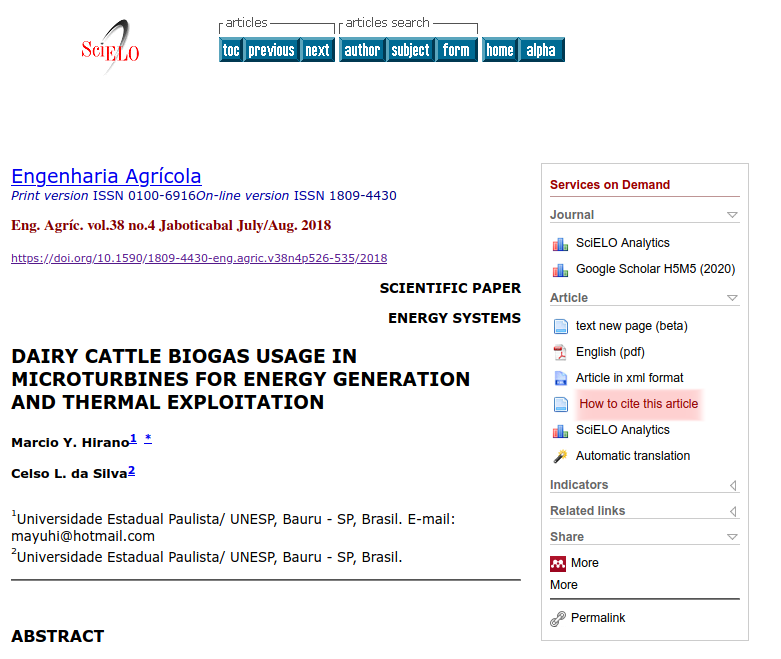
\includegraphics[scale=0.5]{scielo}
\end{center}
Onde, através desta opção, inúmeras maneiras irão aparecer, basta clicar em \textbf{Export to BibTex}.
\begin{center}
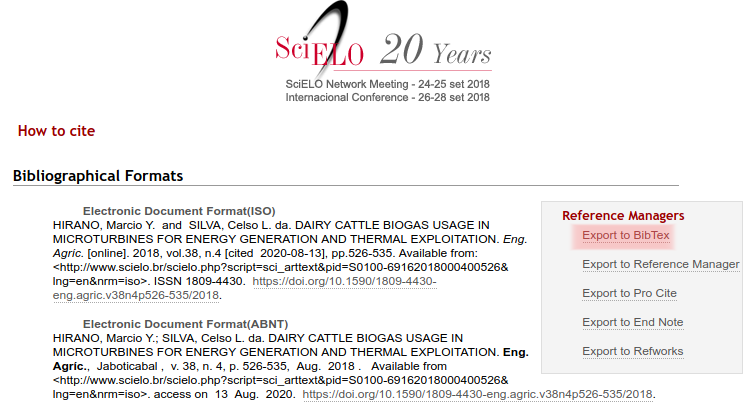
\includegraphics[scale=0.5]{scielo2}
\end{center}
Uma código semelhante a este irá aparecer,
\begin{verbatim}
@article{citacao1,
   title = {COMO UTILIZAR O FACEBOOK PARA VENDER PIA DE BANHEIRO}
   journal = {Um jornal nada aleatorio},
   author={Facebook, BOT},
   ISSN = {00000000000-1},
   language = {en},
   URL = {urlqualquer},
   volume = {38},
   year = {2018},
   month = {08},
   pages = {526 - 535},
   publisher = {sol},
   crossref = {referencia},
   }
\end{verbatim}
Deve-se colocar esta citação na biblioteca de citações e utilizar no texto.
\begin{verbatim}
De acordo com \citeonline{citacao1} é possível entender que \ldots
\end{verbatim}
De acordo com \citeonline{citacao1} é possível entender que \ldots E a entrada de citação será automaticamente feita.\\
Outra forma, pelo Google Acadêmico, é através das aspas de citação.
\begin{center}
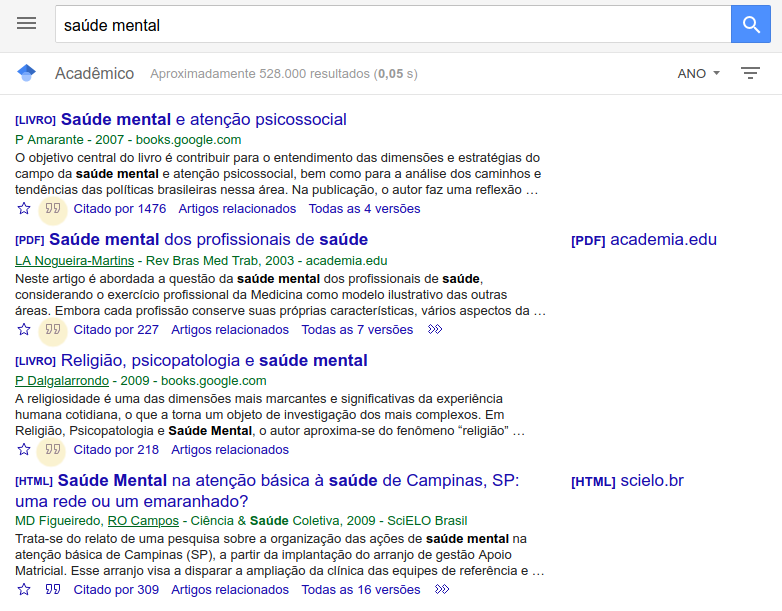
\includegraphics[scale=0.5]{scholar}
\end{center}
Da mesma forma que no scielo, basta clicar em BibTex e incluir o código na base de referências.
\begin{center}
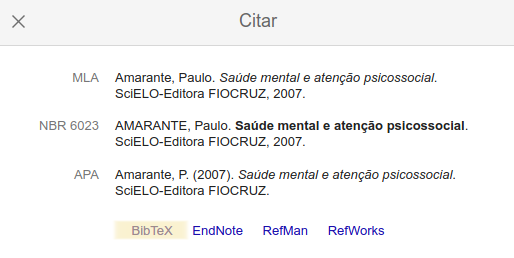
\includegraphics[scale=0.5]{scholar2}
\end{center}
\begin{verbatim}
@book{amarante2007saude,
  title={Sa{\'u}de mental e aten{\c{c}}{\~a}o psicossocial},
  author={Amarante, Paulo},
  year={2007},
  publisher={SciELO-Editora FIOCRUZ}
}
\end{verbatim}
Para citar, basta utilizar o conhecimento já adquirido e utilizar \verb|{\cite{nome da citação}|.
Desta forma, para \citeonline{amarante2007saude}, a psicologia leva o indivíduo a \ldots
Novamente, para finalizar o pdf, a sequência que deve ser seguida é a seguinte:
Os comandos para que as referências sejam dadas, estão a seguir:
\begin{verbatim}
Pressione F6(gerando o pdf),F11 para ler o .bib, 
F6 e F7(para mostrar o arquivo final em pdf).
\end{verbatim}
Se sua referência não aparecer, execute mais de uma vez.
Algumas formas de citação estão expressas abaixo.
\begin{multicols}{2}
\footnotesize
\begin{verbatim}
avaliação e manipulação do
repertório de comportamentos
de indivíduos, de acordo com
\citeonline{pernalonga}.
\end{verbatim}
\ldots avaliação e manipulação do repertório de\\
comportamentos de indivíduos, de acordo com\\
\citeonline{pernalonga}.
\end{multicols}

\begin{multicols}{2}
\footnotesize
\begin{verbatim}
\citeonline[p.-68]{pernalonga}
se selecciónó una 
cohorte de 111 pacientes \ldots
\end{verbatim}
\citeonline[p.-68]{pernalonga}
se selecciónó una 
cohorte de 111 pacientes \ldots
\end{multicols}

\begin{multicols}{2}
\footnotesize
\begin{verbatim}
\ldots impactos do novo conhecimento 
trazido pelas instituições endógenas 
\cite{pernalonga}
\end{verbatim}
\ldots impactos do novo conhecimento 
trazido pelas instituições endógenas 
\cite{pernalonga}
\end{multicols}

\begin{multicols}{2}
\footnotesize
\begin{verbatim}
\ldots como um ambiente seletivo
\footciteref{pernalonga}
\end{verbatim}
\ldots como um ambiente seletivo
\footciteref{pernalonga}
\end{multicols}